\documentclass[a4paper]{article}

\usepackage{placeins}
\usepackage{multicol}
\usepackage{parskip}
\frenchspacing
\usepackage{indentfirst}
\usepackage{hyperref}
\hypersetup{
    colorlinks,
    citecolor=black,
    filecolor=black,
    linkcolor=black,
    urlcolor=black
}
\usepackage{tabu}
\usepackage{longtable}
\usepackage{polski}
\usepackage[utf8]{inputenc} 
\usepackage{amsmath}
\usepackage[pdftex]{graphicx}

\newcommand{\HRule}{\rule{\linewidth}{0.5mm}}

%relationsTable
\newenvironment{relationsTable}[2]{

\begin{center}
  \begin{longtabu}{|l|l|c|c|}
  
 	  \caption{#1}
  \label{#2}
  \hline
	\large\textbf{Rodzic}&\large\textbf{Dziecko} &\large\textbf{Relacja}&\large\textbf{FK / PK}\\
	\endfirsthead
		
\multicolumn{4}{c}%
{{\bfseries \tablename\ \thetable{} -- Kontynuacja tabeli}} \\
  \hline
  	\large\textbf{Rodzic}&\large\textbf{Dziecko} &\large\textbf{Relacja}&\large\textbf{FK / PK}\\
\endhead	
	
	
\hline \multicolumn{4}{|r|}{{Kontynuacja na następnej stronie}} \\ \hline
\endfoot  
  
\hline
\endlastfoot

}
%relationsTable after
{
	\end{longtabu}
	\end{center}
}



% attributesTable
\newenvironment{attributesTable}[1]
{
\begin{longtabu}{|l|l|}
\caption{Lista atrybutów dla obiektu \textbf{#1}}
 ~\\ \hline
\textbf{Nazwa atrybutu} & \textbf{Typ atrybutu}\\ 
	\endfirsthead
		
\multicolumn{2}{c}%
{{\bfseries \tablename\ \thetable{} -- Kontynuacja tabeli}} \\
  \hline
\textbf{Nazwa atrybutu} & \textbf{Typ atrybutu}\\ 
\endhead		
	
\hline \multicolumn{2}{|r|}{{Kontynuacja na następnej stronie}} \\ \hline
\endfoot  
  
\hline
\endlastfoot

}
% attributesTable after
{
\end{longtabu}
}
% attributesTable end


\title{Programowanie serwerów baz danych}
\author{Paweł Sołtysiak, Marcin Klepacki}
\date{\today}

\begin{document}
\begin{titlepage}
\begin{center}

% Upper part of the page. The '~' is needed because \\
% only works if a paragraph has started.

\begin{figure}[ht]
\begin{minipage}[b]{0.45\linewidth}
\centering

\includegraphics[width=\textwidth]{tex/zut_logo}

\end{minipage}
\hspace{0.5cm}
\begin{minipage}[b]{0.45\linewidth}
\centering

\includegraphics[width=\textwidth,height=2cm]{tex/wi_logo}

\end{minipage}
\end{figure}

\textsc{\LARGE Programowanie serwerów baz danych}\\[1.5cm]

\textsc{\Large Projekt}\\[0.5cm]

% Title
\HRule \\[0.4cm]
{ \huge \bfseries System bazodanowy\\ zarządzanie zasobami ludzkimi}\\[0.4cm]

\HRule \\[1.5cm]


\begin{minipage}{0.4\textwidth}
\begin{flushleft} \large
\emph{Autorzy:}\\
Paweł \textsc{Sołtysiak}
\end{flushleft}
\end{minipage}
\begin{minipage}{0.4\textwidth}
\begin{flushright} \large
%\emph{Supervisor:} 
~\\
Marcin \textsc{Klepacki}
\end{flushright}
\end{minipage}
~\\[0.5cm]
\begin{minipage}{0.82\textwidth}
\begin{flushleft} \large
\emph{Grupa:}\\
\textsc{I1-32B}
\end{flushleft}
\end{minipage}


\vfill

% Bottom of the page
{\large \today}

\end{center}
\end{titlepage}
\tableofcontents
\section{Cel projektu}
Celem projektu jest opracowanie modelu danych oraz mechanizmów programowania baz danych dla systemu wspomagającego zarządzanie zasobami ludzkimi.

\section{Zakres funkcjonalny}
System ten będzie przechowywał podstawowe informacje, które usprawnią działanie działu kadr w firmie IT. Baza będzie gromadzić informacje o pracownikach, ich kompetencjach, szkoleniach itp.
\subsection{Moduły funkcjonalne}
\begin{itemize}
\item Moduł \textbf{Osoba} -- ewidencja pracowników oraz kandydatów.
\item Moduł \textbf{Szkolenia} -- Lista dostępnych szkoleń, możliwość zapisania pracownika na szkolenie.
\item Moduł \textbf{Stanowisko} -- Hierarchia stanowisk w firmie.
\item Moduł \textbf{Administracja pracownikami} -- Przyznawanie urlopów, odnotowywanie zwolnień lekarskich.
\end{itemize}
\subsection{Kategorie użytkowników systemu i ich uprawnienia (realizowane funkcje)}
\begin{itemize}
\item \textbf{Administrator} -- pracownik działu kadr, posiada pełen dostęp do bazy danych.
\item \textbf{Pracownik} -- możliwość zgłaszania się na szkolenie, oraz składania podania o urlop.

\end{itemize}
\section{Model semantyczny danych}
\subsection{Obiekty rzeczywiste i abstrakcyjne systemu}
\begin{multicols}{2}
\begin{enumerate}


\item Osoba
\item Państwo
\item Miasto
\item Umiejętność
\item Poziom-Umiejętności
\item Typ-Zatrudnienia
\item Historia-Zatrudnienia
\item Firma
\item Uprawnienie
\item Certyfikat
\item Szkolenie
\item Typ-Szkolenia
\item Stanowisko
\item Oddział
\item Dział
\item Urlop
\item Typ-Urlop
\item Umowa
\item Typ-Umowa
\item Stan-cywilny
\item Język-obcy
\item Rodzaj-Znajomości
\item Historia-Edukacji
\item Szkoła
\item Hobby
\end{enumerate}
\end{multicols}
\subsection{Powiązanie między obiektami}
Spis relacji występujących w systemie bazodanowym, znajduje się w tabeli nr \ref{tab:database-relations} na stronie \pageref{tab:database-relations}, przy wykorzystaniu notacji (\emph{min-max})

\begin{relationsTable}{Spis relacji}{tab:database-relations}

%PRACOWNIK
	\hline	
	Miasto & Pracownik &$1:*$ &\texttt{FK}\\	
	\hline		
	Umiejętność & Pracownik  & $M:N$ &  --- \\
	\hline
	Historia-Zatrudnienia & Pracownik & $M:N$  & ---\\
	\hline
	Uprawnienie & Pracownik & $M:N$ & ---\\
	\hline
	Certyfikat & Pracownik & $M:N$ & ---\\
	\hline
	Szkolenie & Pracownik & $M:N$ & ---\\
	\hline
	Stanowisko & Pracownik& $0:*$ &	\texttt{FK}\\
	\hline
	Pracownik  & Urlop  & $0:*$ & \texttt{PK}\\	
	\hline
	Pracownik &  Umowa & $0:1$ & \texttt{PK}\\
	\hline
	Stan-cywilny & Pracownik & $1:*$ & \texttt{FK}\\
	\hline
	Język-obcy & Pracownik & $M:N$ & ---\\
	\hline
	Historia-Edukacji & Pracownik & $M:N$ & --- \\
	\hline
	Hobby & Pracownik & $M:N$ & ---\\
	%PAŃSTWO
	\hline
	Państwo & Miasto & $1:*$ & \texttt{FK}	\\
	%Stanowisko
	\hline
	Stanowisko & Umowa& $1:*$& \texttt{FK}	\\
	\hline
	Dział & Umowa & $1:0$ & \texttt{FK}	\\
	\hline
	Pracownik & Historia-Edukacji & $1:0$ & \texttt{FK}	\\
	%MIASTO
	\hline
	Miasto & Firma & $1:*$ & \texttt{FK}\\
	\hline
	Miasto & Szkoła & $1:*$ & \texttt{FK}\\
		
	%UMIEJĘTNOŚĆ
	\hline
    Umiejętność &  Szkolenie & $1:*$ & \texttt{FK}\\
	
	%Historia-Zatrudnienia
	\hline
	Typ-Zatrudnienia & Historia-Zatrudnienia & $1:*$ & \texttt{PK}\\
	\hline
	Firma & Historia-Zatrudnienia & $1:*$ & \texttt{PK}\\
	\hline
	Pracownik & Historia-Zatrudnienia & $1:*$ & \texttt{PK}\\
	\hline
	Stanowisko & Historia-Zatrudnienia & $1:*$ & \texttt{PK}\\
	
	%SZKOLENIE
	\hline
	Typ-Szkolenia & Szkolenie & $1:*$ & \texttt{FK}\\
	\hline
	Poziom-Umiejętności & Szkolenie & $0:*$ & \texttt{FK}\\
	%Odział
	\hline
	Odział & Dział & $1:*$ &\texttt{FK}\\
	
	%URLOP
	\hline
	Typ-Urlop & Urlop & $1:*$ & \texttt{FK}\\
	
	%UMOWA
	\hline
	Typ-Umowa & Umowa & $1:*$ & \texttt{FK}\\
	
	
	%Historia-Edukacji
	\hline
	Szkoła & Historia-Edukacji & $1:*$ & \texttt{FK}\\
	
	\hline
	Poziom-Umiejętności & Lista-Języków-Obcych & $0:*$ & \texttt{FK}\\

\end{relationsTable}


Spis relacji dla tabel skrzyżowań, znajdują się w tabeli nr \ref{tab:database-crossover} na stronie \pageref{tab:database-crossover}, przy wykorzystaniu notacji (\emph{min-max})

\begin{relationsTable}{Tabele skrzyżowań}{tab:database-crossover}  

 \hline	
	 Pracownik & Lista-Umiejętności & $0:*$ &\texttt{PK}\\	
	 	\hline	
	 Umiejętność & Lista-Umiejętności & $0:*$ &\texttt{PK}\\
	\hline	
	Pracownik & Lista-Historii-Zatrudnienia & $0:*$ &\texttt{PK}\\	
	\hline	
	Historia-Zatrudnienia & Lista-Historii-Zatrudnienia & $0:*$ &\texttt{PK}\\	
	\hline	
	Pracownik &Lista-Uprawnień & $0:*$ &\texttt{PK}\\	
	\hline	
	Uprawnienie &Lista-Uprawnień & $0:*$ &\texttt{PK}\\
	\hline	
	Pracownik &Lista-Certyfikatów & $0:*$ &\texttt{PK}\\	
	\hline	
	Certyfikat &Lista-Certyfikatów & $0:*$ &\texttt{PK}\\	
	\hline	
	Pracownik &Lista-Szkoleń & $0:*$ &\texttt{PK}\\	
	\hline	
	Szkolenie &Lista-Szkoleń & $0:*$ &\texttt{PK}\\	
	\hline	
	Pracownik &Lista-Języków-Obcych & $0:*$ &\texttt{PK}\\	
	\hline	
	Język-Obcy &Lista-Języków-Obcych & $0:*$ &\texttt{PK}\\	
	\hline	
	 Pracownik &Lista-Historii-Edukacji &$0:*$ &\texttt{PK}\\	
	 \hline	
	 Historia-Edukacji &Lista-Historii-Edukacji &$0:*$ &\texttt{PK}\\	
	\hline	
	Pracownik &Lista-Hobby & $0:*$ &\texttt{PK}\\	
	\hline	
	Hobby &Lista-Hobby & $0:*$ &\texttt{PK}\\	
\end{relationsTable}

\subsection{Klucze główne i pozostałe atrybuty}

\begin{attributesTable}{Osoba}
\hline
\underline{Id} & int \\
\hline
Imię & text \\
\hline
Nazwisko & text\\
\hline
Data-Urodzenia & datetime \\
\hline
Miasto-Id & int \\
\hline
Telefon & text\\
\hline
E--mail & text \\
\hline
PESEL & text \\
\hline
Stan-Cywilny-Id & int \\
\hline
Kandydat & bool \\

%Ostatnia linia
\hline

\end{attributesTable}


\begin{attributesTable}{Państwo}
\hline
\underline{Id} & int \\
\hline
Nazwa & text \\
\end{attributesTable}

\begin{attributesTable}{Miasto}
\hline
\underline{Id} & int \\
\hline
Nazwa & text \\
\hline
Państwo-Id & int \\
\end{attributesTable}


\begin{attributesTable}{Umiejętność}
\hline
\underline{Id} & int \\
\hline
Nazwa & text \\
\end{attributesTable}

\begin{attributesTable}{Poziom-Umiejętności}
\hline
\underline{Id} & int \\
\hline
Opis & text \\
\end{attributesTable}

\begin{attributesTable}{Typ-Zatrudnienia}
\hline
\underline{Id} & int \\
\hline
Nazwa & text \\
\end{attributesTable}

\begin{attributesTable}{Historia-Zatrudnienia}
\hline
\underline{Pracownik-Id} & int \\
\hline
Od-kiedy & datetime \\
\hline
Do-kiedy & datetime \\
\hline
\underline{Typ-Zatrudnienia-Id} & int \\
\hline
\underline{Firma-Id} & int \\
\hline
\underline{Stanowisko-Id} & int \\
\end{attributesTable}


\begin{attributesTable}{Firma}
\hline
\underline{Id} & int \\
\hline
Nazwa & text \\
\hline
Miasto-Id & int\\
\end{attributesTable}


\begin{attributesTable}{Uprawnienie}
\hline
\underline{Id} & int \\
\hline
Nazwa & text \\
\end{attributesTable}


\begin{attributesTable}{Certyfikat}
\hline
\underline{Id} & int \\
\hline
Nazwa & text \\
\end{attributesTable}

\begin{attributesTable}{Szkolenie}
\hline
\underline{Id} & int \\
\hline
Nazwa & text \\
\hline
Od-kiedy & datetime\\
\hline
Do-kiedy & datetime\\
\hline
Typ-Szkolenia-Id & int \\
\hline
Poziom-Umiejętności-Id & int \\
\end{attributesTable}

\begin{attributesTable}{Typ-Szkolenia}
\hline
\underline{Id} & int \\
\hline
Nazwa & text \\
\end{attributesTable}


\begin{attributesTable}{Stanowisko}
\hline
\underline{Id} & int \\
\hline
Nazwa & text \\
\end{attributesTable}


\begin{attributesTable}{Oddział}
\hline
\underline{Id} & int \\
\hline
Nazwa & text \\

\end{attributesTable}


\begin{attributesTable}{Dział}
\hline
\underline{Id} & int \\
\hline
Nazwa & text \\
\hline
Oddział-Id & int \\
\end{attributesTable}

\begin{attributesTable}{Urlop}

\underline{Id} & int \\
\hline
Od-kiedy & datetime\\
\hline
Do-kiedy & datetime\\
\hline
Pracownik-Id & int \\
\hline
Urlop-Typ-Id & int \\
\end{attributesTable}

\begin{attributesTable}{Typ-Urlop}
\hline
\underline{Id} & int \\
\hline
Nazwa & text \\
\end{attributesTable}


\begin{attributesTable}{Umowa}
\hline
\underline{Id} & int \\
\hline
Od-kiedy & datetime\\
\hline
Do-kiedy & datetime\\
\hline
Umowa-Typ-Id & int \\
\hline
Stanowisko-Id& int \\
\hline
Pracownik-Id & int \\
\end{attributesTable}


\begin{attributesTable}{Typ-Umowa}
\hline
\underline{Id} & int \\
\hline
Nazwa & text \\
\end{attributesTable}

\begin{attributesTable}{Stan-Cywilny}
\hline
\underline{Id} & int \\
\hline
Nazwa & text \\
\end{attributesTable}

\begin{attributesTable}{Język-Obcy}
\hline
\underline{Id} & int \\
\hline
Nazwa & text \\
\hline
Rodzaj-Znajomości-Id & int \\
\end{attributesTable}



\begin{attributesTable}{Historia-Edukacji}
\hline
\underline{Id} & int \\
\hline
Od-kiedy & datetime \\
\hline
Do-kiedy & datetime \\
\hline
Szkoła-Id & int \\
\hline
Pracownik-Id & int \\
\end{attributesTable}

\begin{attributesTable}{Szkoła}
\hline
\underline{Id} & int \\
\hline
Nazwa & text \\
\hline
Miasto-Id & int\\
\end{attributesTable}

\begin{attributesTable}{Hobby}
\hline
\underline{Id} & int \\
\hline
Nazwa & text \\
\end{attributesTable}


\begin{attributesTable}{Lista-Umiejętności}
\hline
\underline{Pracownik-Id} & int \\
\hline
\underline{Umiejętność-Id} & int \\
\hline
\underline{Poziom-Umiejętności-Id} & int \\
\end{attributesTable}




\begin{attributesTable}{Lista-Uprawnień}
\hline
\underline{Pracownik-Id} & int \\
\hline
\underline{Uprawnienie-Id} & int \\
\hline
Ważność & datetime \\
\end{attributesTable}

\begin{attributesTable}{Lista-Certyfikatów}
\hline
\underline{Pracownik-Id} & int \\
\hline
\underline{Certyfikat-Id} & int \\
\hline
Kto-Wystawił & text \\
\end{attributesTable}

\begin{attributesTable}{Lista-Szkoleń}
\hline
\underline{Pracownik-Id} & int \\
\hline
\underline{Szkolenie-Id} & int \\
\end{attributesTable}

\begin{attributesTable}{Lista-Języków-Obcych}
\hline
\underline{Pracownik-Id} & int \\
\hline
\underline{Język-Obcy-Id} & int \\
\hline
Poziom & int \\
\end{attributesTable}



\begin{attributesTable}{Lista-Hobby}
\hline
\underline{Pracownik-Id} & int \\
\hline
\underline{Hobby-Id} & int \\
\end{attributesTable}

\subsection{Diagram modelu SERM}
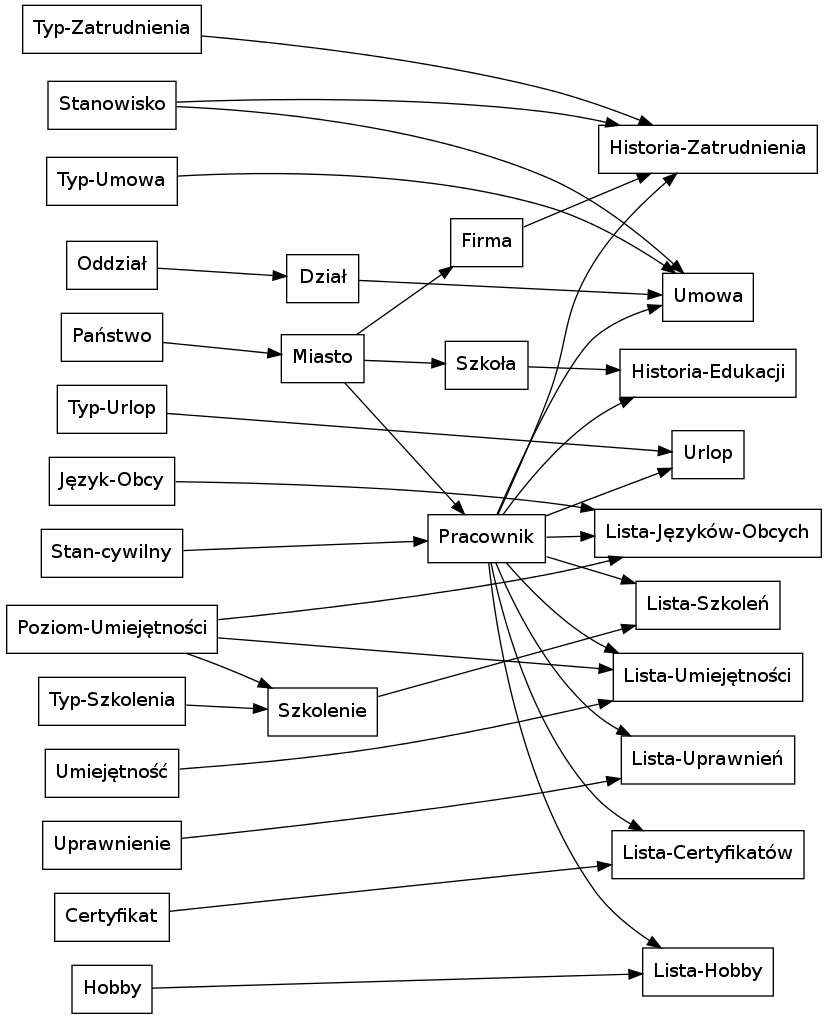
\includegraphics[width=\textwidth]{tex/srem.png}

\end{document}

